\documentclass[aps,reprint,superscriptaddress,nofootinbib, notitlepage,prl]{revtex4-2}

\usepackage[utf8]{inputenc}
\usepackage{graphicx}
\usepackage{xcolor}
\usepackage{mathrsfs}
\usepackage{amsmath}
\usepackage{enumitem}
\usepackage{bm}
\usepackage[colorlinks=true,allcolors=blue]{hyperref}

%to add color text as a comment
\newcommand{\dms}[1]{{\color{blue} #1}}
\newcommand{\cl}[1]{{\color{red} #1}}
\newcommand{\mm}[1]{{\color{teal} #1}}

\bibliographystyle{unsrt}

\frenchspacing
\begin{document}

\title{Connecting anomalous elasticity and sub-Arrhenius structural dynamics in a cell-based model}

\author{Chengling Li}\email{chengling.li@emory.edu}
\affiliation{Department of Physics, Emory University, Atlanta, GA, USA}
\author{Matthias Merkel}
\affiliation{Aix Marseille Univ, Universit\'e de Toulon, CNRS, CPT (UMR 7332), Turing Centre for Living systems,
Marseille, France}
\author{Daniel M. Sussman}\email{daniel.m.sussman@emory.edu}
\affiliation{Department of Physics, Emory University, Atlanta, GA, USA}

\date{\today}

\begin{abstract}
	Understanding the structural dynamics of many-particle glassy systems remains a key challenge in statistical physics.
	Over the last decade, glassy dynamics has also been reported in biological tissues, but is far from being understood.
	It was recently shown that vertex models of dense biological tissue exhibit very atypical, sub-Arrhenius dynamics, and here we ask whether such atypical structural dynamics of vertex models are related to unusual elastic properties.
   It is known that at zero temperature these models have an elasticity controlled by their under-constrained or isostatic nature, but little is known about how their elasticity varies with temperature.
	To address this question we investigate the 2D Voronoi model and measure the temperature dependence of the intermediate-time plateau shear modulus and the bulk modulus. 
	We find that unlike in conventional glassformers, these moduli increase monotonically with temperature until the system fluidizes.
	We further show that the structural relaxation time can be quantitatively linked to the plateau shear modulus $G_p$, i.e.\ $G_p$ modulates the typical energy barrier scale for cell rearrangements.
	This suggests that the anomalous, structural dynamics of the 2D Voronoi model originates in its unusual elastic properties.
	Based on our results, we hypothesize that under-constrained systems might more generally give rise to a new class of ``ultra-strong'' glassformers.
\end{abstract}

\maketitle

%\section{Introduction}

The rheological behavior of disordered materials, in particular in the presence of thermal fluctuations, is still not fully understood.
In the athermal (zero-temperature) limit, it depends strongly on the Maxwell constraint-counting criterion \cite{Maxwell1864,Calladine1978,lubensky2015phonons}, which distinguishes three classes of systems.
Roughly, ``over-constrained'' systems have more constraints than degrees of freedom and are generally rigid.
Conversely, ``under-constrained'' systems have fewer constraints than degrees of freedom and are generally mechanically unstable.
Finally, ``isostatic'' systems have balanced constraints and degrees of freedom, and often behave as weak solids. For disordered materials, this straightforward constraint counting is then modified by non-affine contributions to the systems elasticity \cite{lemaitre2006sum,zaccone2011approximate}.


\begin{figure}[b]
	\centering
	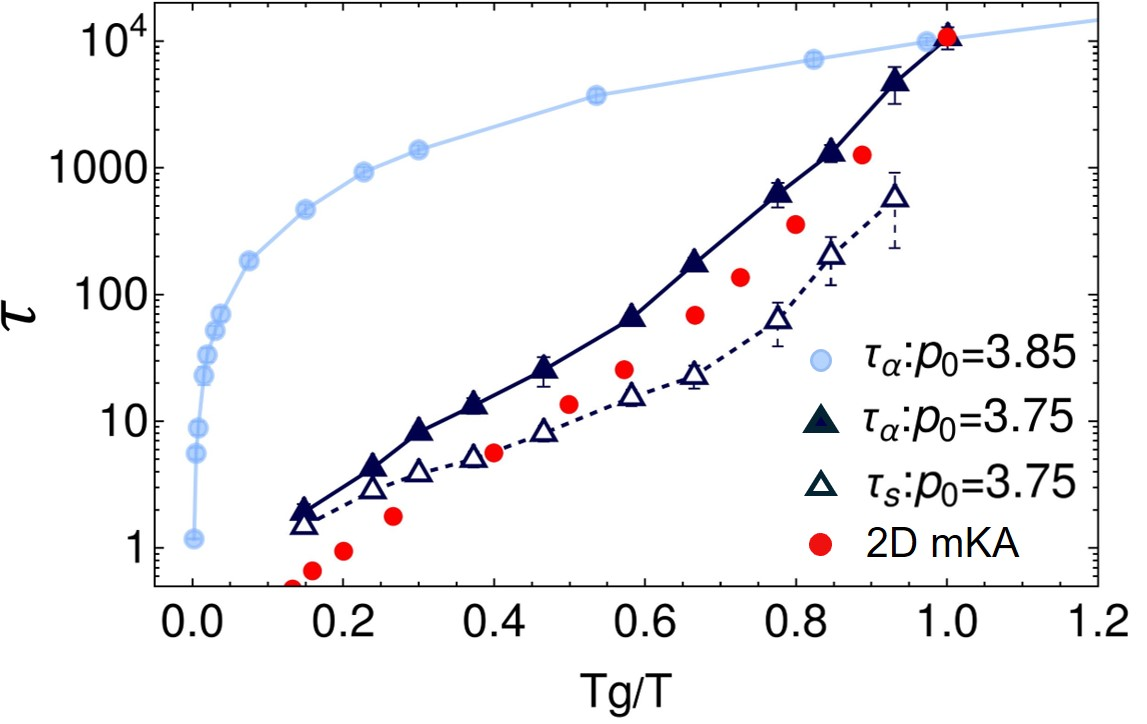
\includegraphics[width=1\linewidth]{tauAlphaPlot.jpg}
	\caption{\textbf{Structural relaxation in the 2D Voronoi model}.
    Scaling of $\tau_\alpha$ of the 2D Voronoi model in the weak solid regime (light blue) and deeper in the solid regime (black), along with data from Ref.~\cite{li2019long} for a standard 2D Kob-Andersen glassformer (red dots). Open symbols show the stress relaxation time, $\tau_s$. Both $\tau_\alpha$ and $\tau_s$ were quantified using standard approaches (see End Matter).
	}
	\label{fig:tauAlphaFig}
\end{figure}

Over-constrained systems, which typically show glassy behavior, are the most well-understood.
Increasing temperature $T$ above the dynamical glass transition temperature $T_g$ facilitates particle rearrangements, which occur on a structural relaxation time scale $\tau_\alpha$.
A simple picture of structural relaxation based on temperature-independent energy barriers of order $\Delta E$ would predict that $\tau_\alpha\sim\exp{(\beta\Delta E)}$, where $\beta = (k_B T)^{-1}$ is the inverse temperature.
Such an exponential scaling of $\tau_\alpha$ with inverse temperature is called Arrhenius scaling, and standard particulate glasses display Arrhenius scaling or super-Arrhenius scaling (in which $\tau_\alpha$ grows faster than exponentially with the inverse temperature, c.f.\ the red dots in Fig.~\ref{fig:tauAlphaFig}) \cite{ediger1996supercooled}.
A long-standing idea is that since particle rearrangements require local elastic deformations of the material $\Delta E$, and thus $\tau_\alpha$, should be connected to elasticity \cite{cavagna2009supercooled,dyre2012instantaneous,puosi2012communication}.
Above $T_g$ at long times the shear relaxation modulus $G(t)$ vanishes and glasses are fluid, but this is often preceded by an intermediate-time plateau with value $G_p$.
Because transient deformations cost energy, the prediction of the elastic or ``shoving'' models is that $\Delta E\sim G_p$, i.e.\ \cite{dyre2012instantaneous,puosi2012communication}:
\begin{equation} 
    \tau_\alpha \sim \exp \left(\beta C G_p\right),\label{eq:shoving} 
\end{equation}
where $C$ is a constant.
In particulate glasses and other over-constrained systems $G_p$ typically varies extremely modestly with temperature, which would be consistent with Arrhenius behavior.
Super-Arrhenius behavior can arise from a slightly larger temperature dependence of $G_p(T)$ which can in turn originate from subtle changes to the inherent states sampled as $T$ changes.

Under-constrained systems are less well understood.
The most commonly studied under-constrained systems have fixed connectivity, such as spring or fiber networks \cite{Merkel2019,chen2024field,broedersz2011criticality}.
While generally floppy at $T=0$, these systems can be rigidified through external strain or by varying model parameters in a way that introduces geometric incompatibility and prestresses.
These prestresses in turn govern elastic properties such as the shear modulus.
There is relatively little work on the thermal behavior of such systems.
A few specific networks have been studied, where the shear modulus was found to scale as a power law with temperature, $G\sim T^\alpha$, for $0.5\leq \alpha \leq 1$ \cite{mao2015mechanical,zhang2016finite}.
Recent analytical work by one of us on generic under-constrained networks found that for small temperatures there are three regimes; an energetically dominated regime with $\alpha=0$ close to the athermal rigid regime, an entropically dominated regime with $\alpha=1$ close to the athermal floppy regime, and a cross-over regime with $\alpha=0.5$ \cite{lee2023generic,lee2023partition}.
Thus, the shear modulus generally \emph{increases} with temperature.
However, because these models have fixed connectivity, no structural relaxation takes place.


There are also under-constrained models whose connectivity is not fixed, for instance ``vertex models'' of dense biological tissue.
These models describe a monolayer of cells as a tiling of polygonal cells \cite{farhadifar2007influence,alt2017vertex,honda1983geometrical}, in which the degrees of freedom are the positions of the polgon corners (i.e., the polygonal vertices).
In a standard implementation of the model, the forces on the vertices are given by the negative gradient of an energy functional with dimensionless form \cite{farhadifar2007influence}:
\begin{equation}\label{eq:cellenergyReduced} 
	E = \sum_{i=1}^{N}\Big[(a_i-1)^2 + (p_i-p_0)^2\Big].
\end{equation}
Here $N$ is the total number of cells, and $a_i$ and $p_i$ are the area and perimeter of cell $i$.
The model parameter $p_0$ corresponds to the target cell perimeter.
For simplicity, parameters corresponding to the preferred cell area, and the area and perimeter stiffness of the cells, have been set to unity.
This form is often motivated biologically --- the area term represents the resistance of the cells to volumetric changes, and the perimeter term represents a competition between active cellular tensions and inter-cellular adhesion \cite{honda1983geometrical,farhadifar2007influence} --- but it can also be view more generically as a low-order expansion in simple geometric quantities \cite{kim2018universal}.
Vertex models have been used to describe many experiments on biological tissues, including observations of cellular jamming transitions and glassy dynamics \cite{schoetz2013glassy,angelini2011glass,sadati2013collective,park2016collective,oswald2017jamming,park2015unjamming,garcia2015physics,tang2022collective,devany2021cell,grosser2021cell}.

Like under-constrained systems with fixed connectivity, athermal vertex models have a rigidity transition \cite{farhadifar2007influence,bi2015density,merkel2018geometrically,Merkel2019,duclut2021nonlinear,tong2022linear}. Specifically, vertex models are floppy with a vanishing shear modulus for $p_0>p_0^\ast$ and rigid with a finite shear modulus for $p_0<p_0^\ast$, where the precise value of the transition point $p_0^\ast\sim 3.812$ depends on the network structure \cite{Wang2020}.
There are also isostatic variants of vertex models, such as the 2D Voronoi model \cite{bi2016motility,sussman2018no,Pinto2022}, where the cell shapes are defined by a Voronoi tessellation, and the degrees of freedom are the Voronoi centers $\bm{r}_i$ of the cells.
There is no floppy regime in this model, but its shear modulus strongly decreases with increasing $p_0$, especially in the weakly solid regime $p_0\gtrsim 3.8$ \cite{sussman2018no}.
That is, at $T=0$, the Voronoi model's behavior seems strongly affected by the transition in the standard vertex model.
Importantly, in vertex and Voronoi models structural rearrangements occur as cells are allowed to change their local connectivity, and one of us showed that in the floppy or weak solid regimes, the structural dynamics of these models are of the atypical \emph{sub}-Arrhenius type (blue solid curve in Fig.~\ref{fig:tauAlphaFig}) \cite{sussman2018anomalous}.
In the athermal solid regime, on the other hand, they show a more normal Arrhenius or super-Arrhenius behavior with temperature (black solid curve in Fig.~\ref{fig:tauAlphaFig}) \cite{li2021softness,Pandey2024}.

Are the atypical structural dynamics of these shape-based models of cells related to the unusual elastic properties of under-constrained systems?
Due to its simplicity, we focus on addressing this question for the 2D Voronoi model.
We first measure its plateau shear modulus $G_p$ and its bulk modulus $K$. In the weakly solid regime, we find that both moduli monotonically \emph{increase} with temperature at small $T$.
In contrast, deep in the solid regime we find that $G_p$ is $T$-independent for $T\ll 1$ and decreases slightly for larger $T$.
We then compare this elastic behavior to the shoving model, Eq.~\eqref{eq:shoving}, and find data collapse when using a slightly modified form.
Our findings suggest that the anomalous structural dynamics of the Voronoi model originate in the unusual temperature dependence of its elastic properties.
This also explains why tuning the model from its weak to its deep solid regime leads to a change from sub- to super-Arrhenius structural dynamics \cite{li2021softness}.
Based on this, we expect to more generally observe sub-Arrhenius structural dynamics in under-constrained systems close to the athermal floppy regime.

%\section{Method and model}

We perform standard NVT simulations of the 2D Voronoi model with periodic boundary conditions.
The Voronoi centers $\bm{r}_i$ are subject to forces $\bm{f}_i=-\partial E/\partial\bm{r}_i$, where $E$ is the energy functional in Eq.~\eqref{eq:cellenergyReduced}.
We use the deterministic Nose-Hoover algorithm to control the temperature; in this setting inertia is present and there is no viscous damping that acts on the cell velocities (see End Matter for details).

\begin{figure}[h]
	\centering
	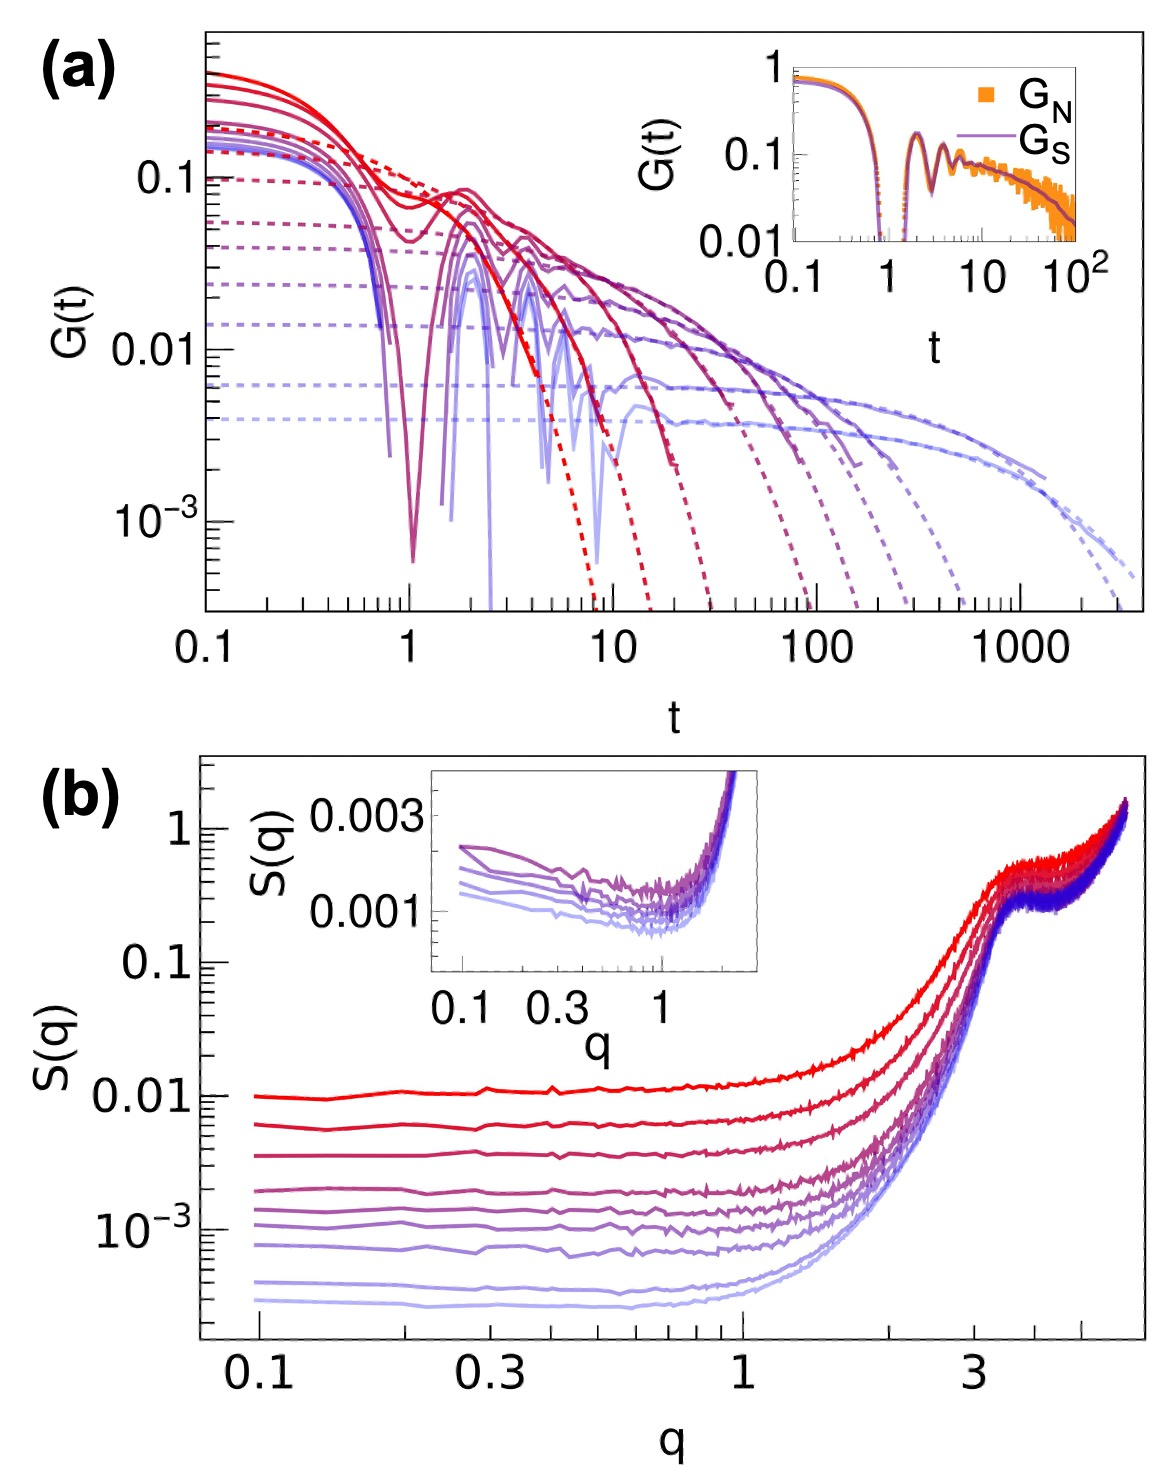
\includegraphics[width=1\linewidth]{GtSq.jpg}
	\caption{\textbf{Stress relaxation and static structure are strongly temperature-dependent}. 
		\textbf{(a)} Shear relaxation modulus as a function of time for $p_0=3.825$ and $T=\left[0.063 - 0.0005\right]$, decreasing from dark red to light blue.
		Dashed lines are stretched exponential fits.
		Inset: $G(T)$ at $T=0.0025$ computed via stress autocorrelations ($G_S$) or a small step strain ($G_N$).
		\textbf{(b)} The isotropic static structure factor $S(q)$ for $p_0=3.825$ and the same range of temperatures as in (a). 
		Inset: $S(q)$ for $p_0=3.8$ at $T=0.00385, 0.0031, 0.0028, 0.0025, 0.0022$.
	}
	\label{fig:GtSq}
\end{figure}

We first quantify the plateau shear modulus $G_p$.
To this end, we compute $G(t)$ via the shear stress auto-correlation function (see End Matter).
Figure~\ref{fig:GtSq}(a) shows sample $G(t)$ curves across a range of $T$ for $p_0=3.825$.
We independently verified these results by measuring $G(t)$ from the stress response to a small shear step (Fig.~\ref{fig:GtSq}(a) inset).
We find that the magnitude of $G(t)$ is strongly temperature-dependent at almost all time scales (Fig.~\ref{fig:GtSq}(a)).
As $T$ decreases, similar to other glassy systems \cite{flenner2019viscoelastic,puosi2012communication}, an intermediate-time plateau gradually emerges, followed by a final decay.
We quantify $G_p$ and the duration $\tau_s$ of the intermediate-time plateau by fitting our $G(t)$ data to a stretched exponential form, $G(t)\approx G_p e^{-(t/\tau_s)^\beta}$ at intermediate and late times (dashed curves in Fig.~\ref{fig:GtSq}(a), see End Matter).
We find that $\tau_s$ is typically several times smaller than $\tau_\alpha$ (Fig.~\ref{fig:tauAlphaFig}), suggesting that in this model stress-bearing structures can dissipate before individual cells move a substantial amount.

\begin{figure}[b]
	\centering
	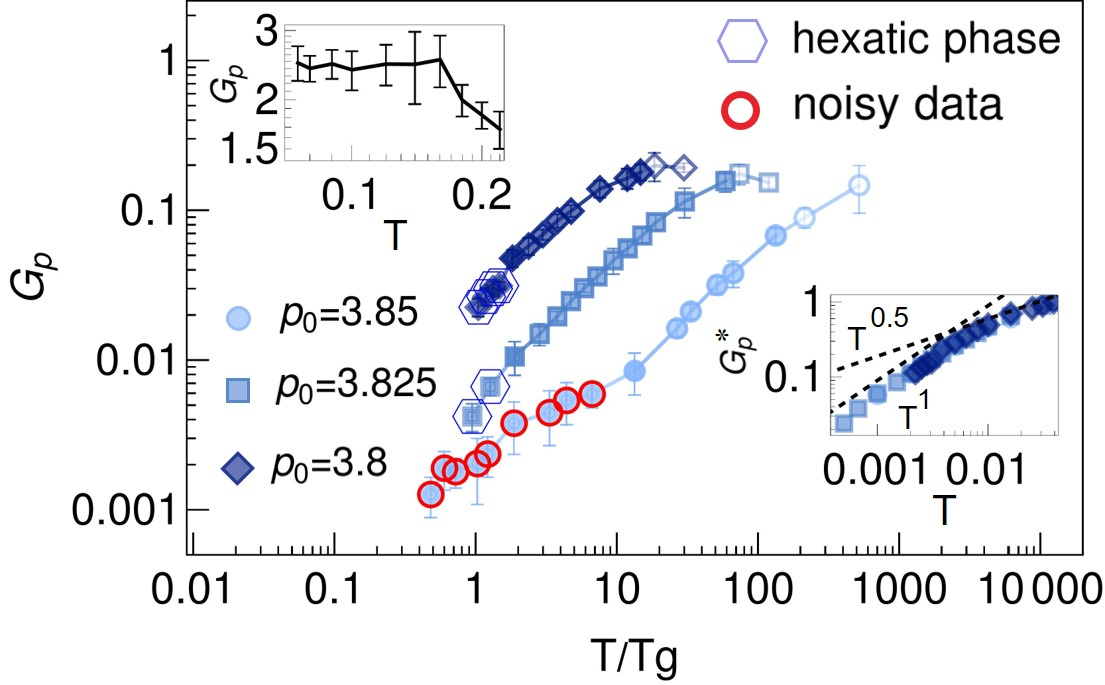
\includegraphics[width=1\linewidth]{Gp.jpg}
	\caption{\textbf{The plateau shear modulus $G_p$ is strongly temperature-dependent.}
		Here state points corresponding to the hexatic phase are plotted by shown with a hexagon.
		At the lowest temperatures for $p_0=3.85$, the tail of $G(t)$ is both noisy and poorly fit by a stretched exponential; we consider these measurements less reliable and note them with red open circles.
		Lower Inset: $G_p^*=G_p/G_p(T=0.039)$ for each $p_0$ as a function of $T$.
		Dashed lines are guides to the eye of slope 1 and $1/2$.
        Upper Inset: $T$-dependence of a $p_0=3.0$ Voronoi model whose structural relaxation is super-Arrhenius \cite{li2021softness}.
    }
	\label{fig:gpT}
\end{figure}

In Fig.~\ref{fig:gpT}, we plot the plateau shear modulus $G_p$ for $p_0=(3.8,3.825,3.85)$ as a function of $T/T_g$, with $T_g$ defined by $\tau_\alpha(T_g)\equiv 10^4$.
In contrast to particulate glassformers \cite{lu2009correlation,flenner2019viscoelastic,puosi2012communication}, in the Voronoi model $G_p$ strongly \emph{increases} upon increasing $T$ until at high enough temperatures we find a pure exponential decay of $G(t)$, which we associate with a fluid phase (Fig.~\ref{fig:gpT}).
At low temperatures the system enters a hexatic phase (hexagons in Fig.~\ref{fig:gpT}), as measured by a peak in the susceptibility of the bond-orientational order parameter \cite{halperin1978theory} -- this is consistent with earlier hexatic-phase observations in vertex models \cite{li2018role}.
Finally, we note that the $G(t)$ data for $p_0=3.85$ at the lowest temperatures was both noisy and poorly fit by a stretched exponential (red dots in Fig.~\ref{fig:gpT}), as we begin to hit the floor associated with the statistical error of our autocorrelator.
We have ignored this data in our subsequent analysis.

As shown in Fig.~\ref{fig:gpT}, for $p_0 \gtrsim 3.8$ $G_p$ monotonically increases with temperature.
In the lower inset we rescale $G_p$ by its value in our highest-$T$ simulations --- we find excellent collapse of our data, with scaling that is consistent with $G_p$ crossing over between $T^1$ and $T^{0.5}$ power laws.
Although our data are over a numerical range to be conclusive, we note that these results are consistent with observations in various fixed-connectivity spring-network models \cite{zhang2016finite,mao2015mechanical,arzash2023mechanical} and those predicted in generic under-constrained systems \cite{lee2023generic,lee2023partition}.

Given that the Voronoi model shows super-Arrhenius behavior deeper in the solid regime, we also measured the plateau shear modulus for the $p_0=3.0$ model studied in \cite{li2021softness} (Fig.~\ref{fig:gpT}, upper inset).
We find that $G_p$ is roughly constant at small temperatures and decreases for larger temperatures. That is, in the regime in which the model's dynamics mirror those of a more typical glassformer, so too does its elasticity.

\begin{figure}[t]
	\centering
	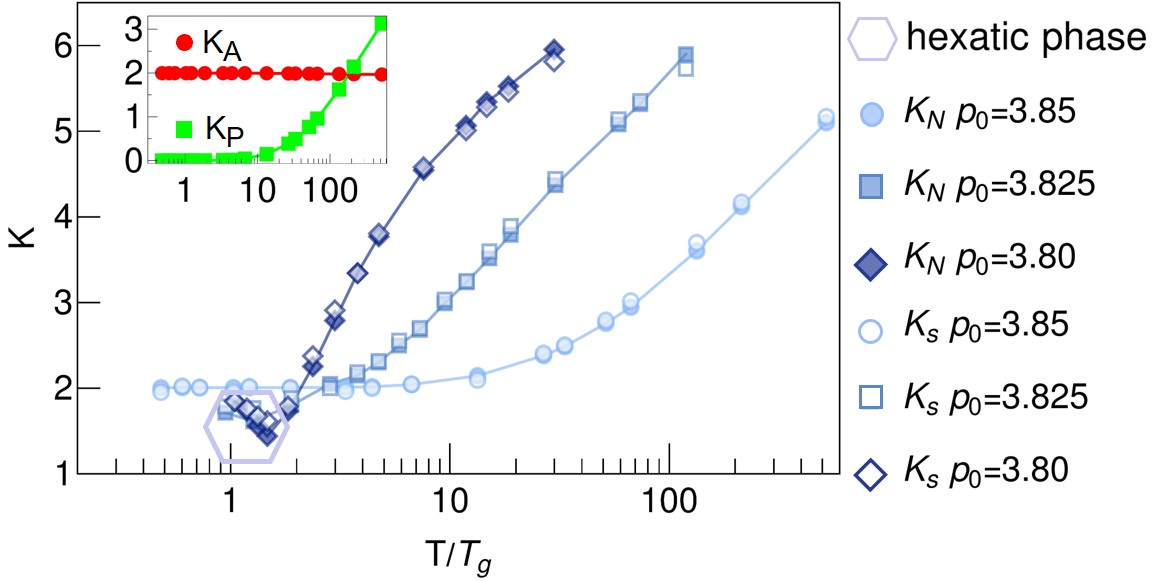
\includegraphics[width=1\linewidth]{K.jpg}
	\caption{\textbf{The bulk modulus $K$ is strongly temperature-dependent.}
		The bulk modulus as calculated from the statis structure factor (open symbols) and the response to isotropic compression (closed symbols).
		Inset: Contributions to $K$ from area ($K_a$) and perimeter ($K_p$) terms in the energy.
	}
	\label{fig:K}
\end{figure}

We also characterize the temperature dependence of the bulk modulus $K$ from the low-wavevector behavior of the static structure factor (Fig.~\ref{fig:GtSq}(b)), which we also verified by measuring the system response to an isotropic compression strain (see End Matter).
In Fig.~\ref{fig:K}, we plot the bulk moduli obtained through both methods, $K_s$ and $K_N$, as a function of $T/T_g$ for $p_0=(3.8,3.825,3.85)$.
Again in contrast to typical glassy systems, we find that $K$ increases monotonically with $T$: as the system is heated it becomes more resistant to isotropic deformations.
As shown in the inset to Fig.~\ref{fig:K}, this temperature dependence of $K$ comes entirely from cell perimeter contributions to the energy, consistent with work on the athermal transition in vertex models \cite{sussman2018no,Merkel2019}.


\begin{figure}[b]
	\centering
	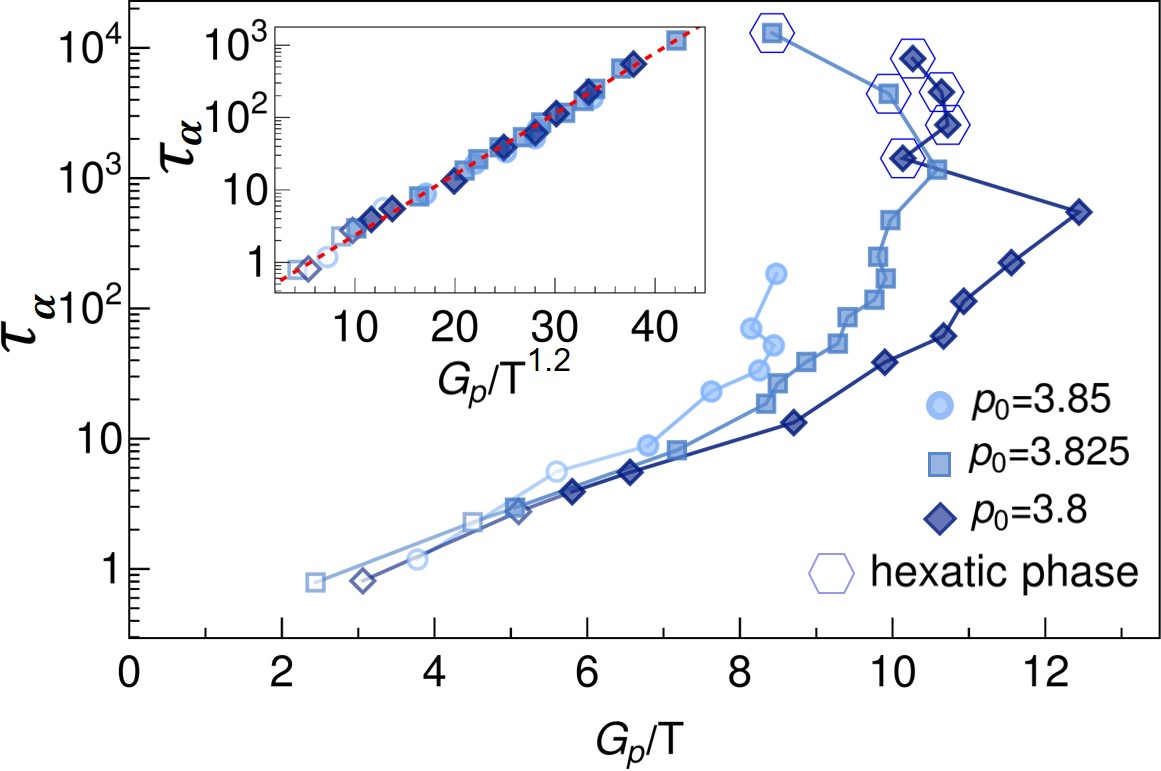
\includegraphics[width=1\linewidth]{connection.jpg}
	\caption{\textbf{The mechanics and dynamics are directly connected.}
		In the main plot we show $\log (\tau_\alpha) \ vs\ G_p/T$; the inset shows $\log (\tau_\alpha) \ vs\ G_p/T^{1.2}$.
		As in plots above, state points corresponding to hexatic phases or unreliable measurements of $G(t\rightarrow\infty)$ are noted. 
	}
	\label{fig:connection}
\end{figure}

Given the unusual temperature dependence of the Voronoi model's elastic moduli, does a shoving model such as Eq.~\eqref{eq:shoving} explain the anomalous structural dynamics?
In Fig.~\ref{fig:connection} we plot $\log(\tau_\alpha)$ vs. $G_p/T$ for the weak solid regime and find neither a linear scaling nor a compelling collapse of the data.
However, the inset shows excellent collapse by instead scaling $G_p$ by $T^{1.2}$.
This deviation from the typical elastic model suggests the presence of some other very modestly temperature-dependent feature contributes to the energy barrier $\Delta E$.

%\section{Discussion}


In summary, we have shown that the atypical sub-Arrhenius structural dynamics in the 2D Voronoi model is directly correlated to the unusual temperature dependence of its elastic moduli.
We specifically found that in the weak solid regime the plateau shear modulus monotonically increases with temperature, in a way which is qualitatively consistent with analytical results on fixed connectivity under-constrained systems \cite{lee2023generic,lee2023partition}.
Although the 2D Voronoi model is isostatic rather than under-constrained, we note that at $T=0$ the elastic moduli of the Voronoi model have been shown to be governed by the rigidity transition of the vertex model \cite{sussman2018no}.
Additionally, we note that the structural dynamics of the 2D vertex model is known to be similar to that of the 2D Voronoi model \cite{sussman2018anomalous}, and the finite-temperature behavior is expected to be extremely similar to what we report here for the Voronoi model \cite{lee2023generic,lee2023partition}.
%Second, in the deep solid regime of the 2D Voronoi model the structural dynamics becomes more conventional (black solid curve in Fig.~\ref{fig:tauAlphaFig}) \cite{li2021softness}, consistent with its constant plateau shear modulus in this regime (Fig.~\ref{fig:gpT}, upper inset); this in turn follows the prediction of a temperature-independent shear modulus in the solid regime of under-constrained systems \cite{lee2023generic,lee2023partition}.
%Finally, in the 2D vertex model, the structural dynamics is known to be similar to that of the 2D Voronoi model \cite{sussman2018anomalous}, and the finite-temperature behavior of the elastic moduli close to the athermal fluid regime is expected to be extremely similar to what we report here for the Voronoi model \cite{lee2023generic,lee2023partition}.
Taken together, we expect that the reported sub-Arrhenius structural dynamics of the 2D vertex model is also explained by its elastic properties in the large-$p_0$ regime.
In the small-$p_0$ regime, in contrast, the more conventional structural dynamics \cite{Pandey2024} are likely related to the predicted more conventional elastic properties \cite{lee2023generic,lee2023partition}.

More generally, we expect this scenario --- unusual elasticity connected to anomalous structural dynamics close to the athermal fluid regime, and more conventional elasticity and structural dynamics in other parts of parameter space --- to appear in any under-constrained system that is allowed to dynamically change its connectivity.
To our knowledge the only class of systems with glassy behavior similar to the vertex model are low-density vitrimeric polymers \cite{ciarella2019understanding}, where a network of covalently bonded under-constrained monomers can change its connectivity on long time scales via bond-exchange reactions.
We suggest that models with similar thermally dependent elasticity may all form a class of ``ultra-strong'' glasses, complementing the currently classification of ``fragile'' and ``strong'' glassformers.
If true, our findings may help to develop new materials with such an ultra-strong glass-forming ability.

Finally, our results have implications for the modeling of biological tissues.
Some modeling of dense tissue uses not shape-based under-constrained models but more typical particle-based models \cite{Germann2019,Henkes2020}.
Given the differences in elastic and structural properties between particulate glasses and vertex models, our work shows how this choice can lead to fundamentally different tissue-scale behavior.
For instance, under certain conditions, e.g.,\ when the auto-correlation time of cell motile forces are smaller than any other relevant time scale of the system, cell motility may be approximated by thermal noise. For such systems, our findings suggest that an increase in cellular motility would not only fluidify the tissue on long times \cite{bi2016motility}, but may also \emph{increase} the intermediate-time, tissue-scale rigidity ($G_p$).
It would be interesting to test this experimentally.

\begin{acknowledgments}
This material is based upon work supported by the National Science Foundation under Grant No.~DMR-2143815 (DMS and CL). 
This research used the Delta advanced computing and data resource which is supported by the National Science Foundation (award OAC 2005572) and the State of Illinois. Delta is a joint effort of the University of Illinois Urbana-Champaign and its National Center for Supercomputing Applications.
\end{acknowledgments}

\bibliography{finiteTemperatureMechanics}

\appendix

\section{End Matter}

\subsection{Simulation details}

We perform standard NVT simulations~\cite{martyna1996explicit,frenkel2002understanding} of the 2D Voronoi model under periodic boundary conditions using the open-source \emph{cellGPU} package~\cite{sussman2017cellgpu}. Temperature is controlled by coupling the system to a Nose-Hoover thermostat with fictitious degrees of freedom $\zeta_i$. The equations of motion of the standard Nose-Hoover thermostat are
\begin{align}
    m_i \ddot{\bm{r}}_i &= \bm{f}_i - \zeta m_i \bm{v}_i\\
    \dot{\zeta} &= Q^{-1} \sum_i^N m_i v_i^2 - N_f k_BT,
\end{align}
where $m_i$ and $\bm{v}_i$ are the mass and velocity of particle $i$, $N_f$ is the number of degrees of freedom in the system, $T$ is the target temperature, and $Q$ is the thermostat parameter that determines its relaxational dynamics. This non-Hamiltonian scheme is one of the most accurate and efficient ways of simulating a constant-temperature ensemble, and we further make use of a formulation with a short chain of fictitious thermostat variables \cite{martyna1996explicit}. We then employ for each timestep a standard update of the equations of motion based on a Trotter factorization \cite{frenkel2002understanding}.

We measure the characteristic relaxation time, $\tau_\alpha$, by measuring the decay of the cage-relative self-intermediate scattering function $F^{CR}_s$ \cite{vivek2017long, illing2017mermin}.
We ensure that all simulations have been equilibrated for at least $10$ times longer than the measured $\tau_\alpha$.
We report results for systems of $N=4096$ cells, and have checked that increasing this to $N=32768$ does not change our results.

\subsection{Unusual cage dynamics at short times}

We note that the shear relaxation modulus shown in Fig.~\ref{fig:GtSq} has substantially more structure at short times than is usually seen in glassforming systems.
This is a direct reflection of the unusually large cage fluctuations, in which cells undergo surprisingly large displacements without exchanging neighbors, that characterize single-particle motion in these models.
This can also be seen in the unusual behavior of the scattering function itself. 
As shown in Fig.~\ref{fig:cageRelativeFs}, one sees that the initial plateau of $F^{CR}_s$ is itself substantially lower than in particulate systems, indicating that a large number of cells move substantially but not so far that they escape their cage and keep diffusing.
Furthermore, there is evidence of a secondary relaxation process (the minima and non-monotonicity after the initial decay) indicative of ``cage-rebounding'' dynamics. This process itself has a characteristic temperature dependence.

\begin{figure}[t]
	\centering
    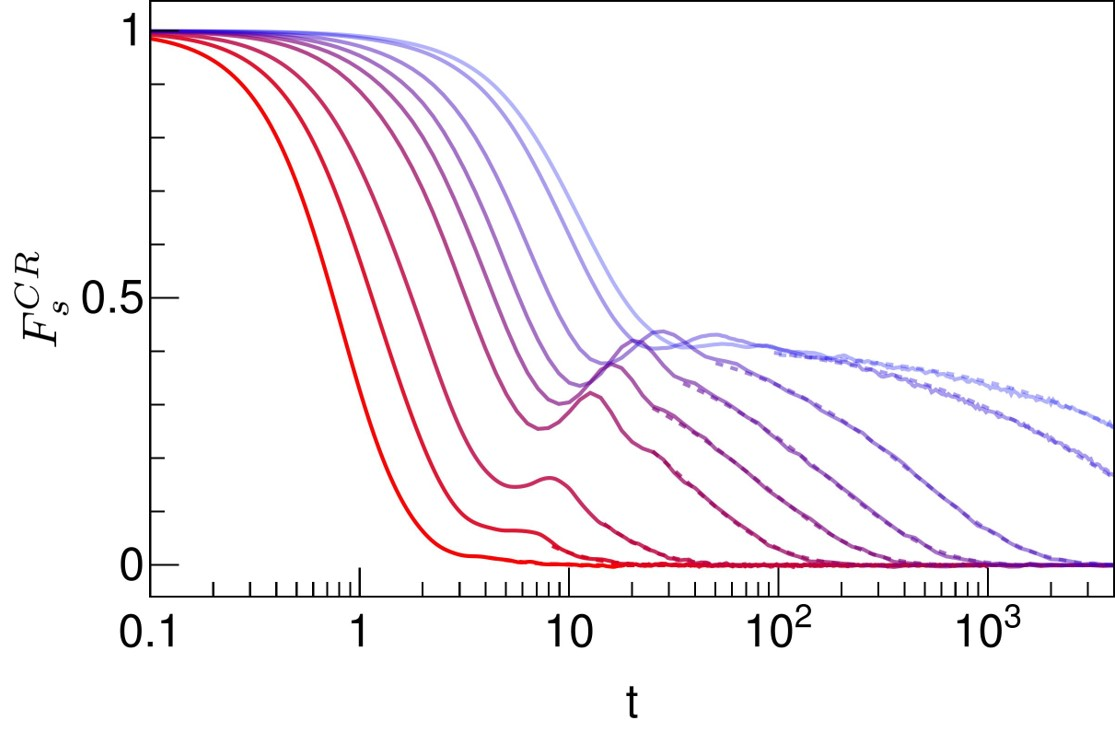
\includegraphics[width=.9\linewidth]{endMatter_CageRelativeFs}
	\caption{\textbf{The cage-relative scattering function $F^{CR}_s$ shows unusual cage dynamics.}
        Curves correspond to the same systems ($p_0$ and $T$) as in Fig.~\ref{fig:GtSq}, and the scattering function is measured at a wavevector corresponding to the first peak of the structure factore.
	}
	\label{fig:cageRelativeFs}
\end{figure}

\subsection{Quantification of the plateau shear modulus}

At each simulation step we analytically calculate the shear stress $\sigma_{xy}\equiv (\mathrm{d}E/\mathrm{d}\gamma)/A$, where $\gamma$ is the shear strain deforming the periodic box, and $A$ is the total system area.
We then compute $G(t)$ via the stress auto-correlation function 
\begin{equation}\label{eq:G(t)}
	G(t)=\frac{A}{k_BT}\Big\langle\sigma_{xy}(t_0)\sigma_{xy}(t_0+t)\Big\rangle,
\end{equation}
where $\langle...\rangle$ represents an average over $t_0$ for each simulation, with statistics accumulated using a multiple-tau correlator method \cite{ramirez2010efficient}.

We verified these results by independently measuring $G(t)$ from the response to a small shear step $\Delta \gamma$ at $t=0$ via $G(t)=\Delta \sigma_{xy}(t)/\Delta\gamma$. Specifically, we imposed a pure shear deformation on the orthonormal shape of the primary unit cell, numerically measured the derivative of energy with respect to this pure shear deformation, and converted the pure shear modulus to the simple shear modulus, $G$.

We obtain $G_p$ and $\tau_s$ by fitting $G(t)$ to a stretched exponential form, $G(t)\approx G_p e^{-(t/\tau_s)^\beta}$ at intermediate and late times.
More precisely, we fit data from $10$ simulations for $t\in \left[t_i,t_f\right]$ for each set of parameters $(p_0,\ T)$; $t_i$ is chosen as the earliest time that an approximate plateau appears. If there is no such plateau, we vary $t_i$ across a range to ensure a qualitatively good fit encompassing as many data points as possible. We choose $t_f$ as the time at which the magnitude of $G(t)$ is comparable to either the thermal fluctuations or the statistical error of our autocorrelation method \cite{ramirez2010efficient}.

\begin{figure}
	\centering
    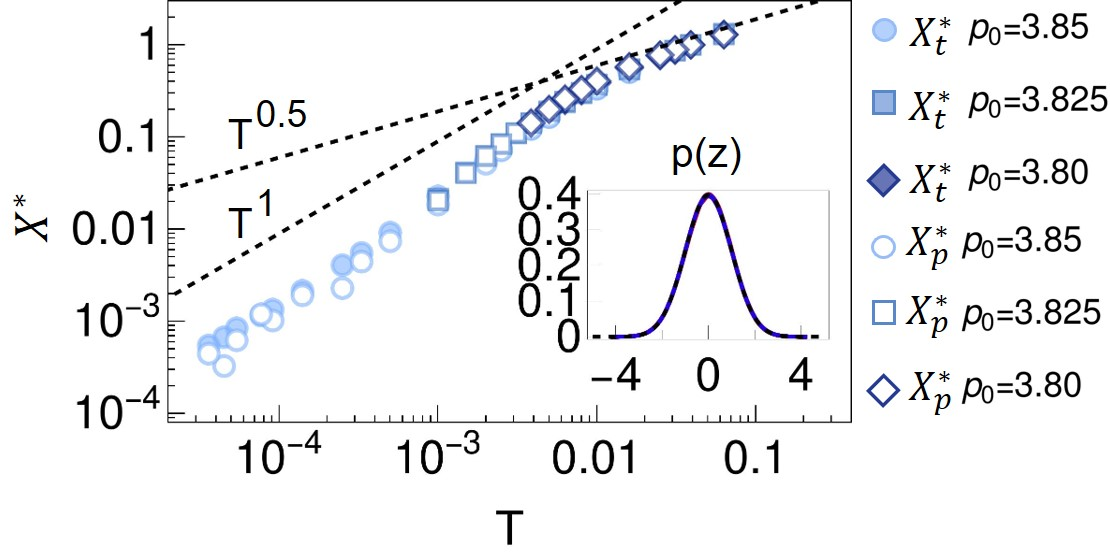
\includegraphics[width=1\linewidth]{endMatter_tension.jpg}
	\caption{\textbf{Scaling of perimeter-related contributions to the energy with temperature.}
        The main plot shows the behavior of $X_t^\ast$ (the mean cell tensions) and $X_p^\ast$ (the average deviation of cell perimeters from their preferred value) at different values of $p_0$.
        The inset shows the probability density function of standardized cell perimeters (i.e., $z=(p-\mu)/\sigma$) --- as shown, these distributions are extremely close to Gaussian.
	}
    \label{fig:tension}
\end{figure}

Intuitively, previous work by one of us suggests that the ``entropic elasticity'' behavior of the shear modulus stems from changes in the accessible volume of phase space as the perimeter increases above $p_0^\ast$. In this regime, higher temperatures favor larger mean values of the actual cell perimeters, which in turn imply monotonically increasing perimeter tensions.
These tensions are in turn what rigidifies the system.
We present data for this in Fig.~\ref{fig:tension}, which shows the scaling of both $\langle p-p_0\rangle$ and the average cell tensions, $t=(\sigma_{xx}+\sigma_{yy})/2$ as a function of temperature.
We find good agreement with the theoretical expectations based on generic underconstrained systems \cite{lee2023generic,lee2023partition}, and a high correlation between this measurement and the data on $G_p(T)$ itself presented in Fig.~\ref{fig:gpT}.
Although the plateau shear modulus is \emph{dominated} by perimeter contributions, we note that we do measure non-zero contributions from the area elasticity to the stress autocorrelation function.


\subsection{Quantification of the bulk modulus}
We quantify the bulk modulus $K$ by measuring the low-wavevector behavior of the static structure factor, $S(\textbf{q}) \equiv \frac{1}{N}\sum_{j=1}^{N}\sum_{k=1}^{N} e^{- i\textbf{q}\cdot (\textbf{r}_j-\textbf{r}_k)}$, where $j,k$ index the cells.
The bulk modulus is $K_s=Nk_BT/AS(q\rightarrow 0)$ \cite{hansen2013theory,zhuravlyov2023finite}.
Fig.~\ref{fig:GtSq}(b) shows representative plots of $S(q)$ across a range of $T$ for $p_0=3.825$.
For most of our systems there is an unambiguous low-$q$ plateau, although for the lowest temperatures for $p_0=3.8$ there is a non-monotonicity at small $q$ (Fig. \ref{fig:GtSq}(b)).
We thus use the minimum value attained by the structure factor, $S(q_\mathrm{min})$, as a lower bound for $S(q\rightarrow 0)$ at those temperatures.

We verified these results by directly measuring $K$ from the response to an isotropic compression strain of $10^{-3}$, computing the bulk modulus as $K_N=-A \mathrm{d}P/\mathrm{d}A$, for $P=-(\sigma_{xx}+\sigma_{yy})/2$. The greatest deviations between these two measures are in the regime where $S(q)$ has these low-wavevector non-monotonicities and the structure begins hexatically ordering.

\end{document}
